\documentclass[
	12pt, % Default font size, values between 10pt-12pt are allowed
	%letterpaper, % Uncomment for US letter paper size
	%spanish, % Uncomment for Spanish
]{brayton_cycle_report_style}

\usepackage{my_packages}
\usepackage{comment}
\usepackage[inkscapeformat=png]{svg}
\usepackage{subfig}
\usepackage{multicol}
\usepackage[hidelinks,colorlinks=true,linkcolor=blue,citecolor=blue]{hyperref}
\usepackage[font=scriptsize,labelfont=bf]{caption}



%------------------------------------------------------------------------------------

\title{Brayton Cycle Analysis}        % Assignment title
\author{Authors by Last Name: Heath Buer, Joshua Hoffman, McCade Hughes, Bennet Outland}   % Student name
%Partner Name
%\roll{Lorem Ipsum, Lorem Ipsum}                    % Class roll
\class{Thermodynamics II}              % Class
\session{M01/M02}             % Session
\email{\\ heath.buer@mines.sdsmt.edu \\ \\ joshua.hoffman@mines.sdsmt.edu \\  lane.hughes@mines.sdsmt.edu \\ bennet.outland@mines.sdsmt.edu}
\date{\today}        % Due date
\institute{Department of Mechanical Engineering}              % Institute or school name
\course{ME 312}                            % Course or course name
\professor{Dr. Khosro Shahbazi}                                           % Professor or teacher in charge of the assignment

%------------------------------------------------------------------------------------
\addbibresource{ref.bib} 

\setcounter{secnumdepth}{-2} 
%\renewcommand{\thesection}{}  % https://tex.stackexchange.com/a/30202/114006
%------------------------------------------------------------------------------------
\begin{document}
\maketitle 
\begin{table}
    \centering
    \begin{tabular}{c|c}
        Name & \% Effort \\
        \hline
        Heath Buer & 25\% \\
        Joshua Hoffman & 25\% \\
        McCade Hughes & 25\% \\
        Bennet Outland & 25\%
    \end{tabular}
\end{table}





\pagenumbering{gobble}  
\newpage
\pdfbookmark[section]{\contentsname}{toc}
\tableofcontents
\newpage
\pagenumbering{arabic}          % to start the page numbering

%-----------------------------------------
%Requirements
\section{Project Objectives}
This project analyzes different variations of the Brayton Gas Power Cycle to determine the best cycle and working gas for a power plant design. The cycles and gasses are evaluated using the following criteria: the net work produced, first and second law efficiencies, and exergy destroyed. For each criteria, $T_{min}$ and $T_{max}$ of the working gas are held constant; while, the pressure ratio, working gas, component efficiencies, and regenerative effectiveness are varied. Using the results, an optimum Brayton Cycle power plant design is proposed and its components and operating conditions are specified. 

\section{Temperature Parameters}
The low temperature reservoir is selected to be $283K$ $(\approx 10^{\circ} C)$. This was chosen because the Missouri River in South Dakota has a temperature of approximately $0^{\circ} C$ and using it as a low temperature reservoir for a large power plant may increase the temperature a non-trivial amount \cite{commerce_2022}. Due to the increase of temperature to the local surroundings, a reasonable temperature for the working gas is $313K$ $(\approx 40^{\circ} C)$. The high temperature reservoir is selected to be $1620K$, $(\approx 1347^{\circ} C)$. Therefore, a reasonable maximum temperature for the working gas is $1590K$ $(\approx 2400^{\circ} F)$ \cite{general_electric}. The maximum temperature of the working gas is $30^{\circ} C$ lower than the high temperature reservoir due to heat loss to the surroundings.
\section{Brayton Cycle Designs and Working Gases}

The closed Brayton cycles were chosen for analysis because non-air open cycles are expensive. Furthermore, when gasses, other than air, are released into the atmosphere, they have a negative environmental impact. Following an examination of a variety of gasses, Air, Argon, Helium, and Hydrogen were chosen as our working gasses. This is due to their disparate properties which lend distinct comparisons. A table of the properties of the gasses chosen can be seen in Table (\ref{tab:gasses}). Furthermore, the four Brayton Cycles chosen for analysis is shown in Figure (\ref{fig:cycles}). 


\vspace{15mm}

\begin{table}[ht]
    \centering
    \caption{A list of important properties of the gasses used in this investigation.}
    \begin{tabular}{c|c|c|c}
        Gas & $c_{p} \, \left( \frac{kJ}{kg \cdot K} \right)$ & $c_{v} \, \left( \frac{kJ}{kg \cdot K} \right)$ & $\kappa$ \\
        \hline
        Air & 1.005 & 0.718 & 1.400 \\
        Argon ($Ar$) & 0.5203 & 0.3122 & 1.667 \\
        Hydrogen ($H_2$) & 14.307 & 10.183 & 1.405 \\
        Helium ($He$) & 5.1926 & 3.1156 & 1.667
        \label{tab:gasses}
    \end{tabular}
    \label{tab:my_label}
\end{table}


\begin{figure}%
    \centering
    \subfloat[\centering]{{\includegraphics[width=7cm]{figures/cycles/SIMPLE_Brayton_Cycle.png} }}%
    \qquad
    \subfloat[\centering]{{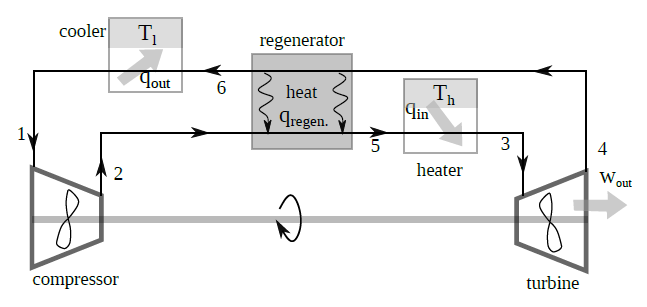
\includegraphics[width=7cm]{figures/cycles/Simple_Brayton_Cycle_Regen.png} }}%
    \qquad
    \subfloat[\centering]{{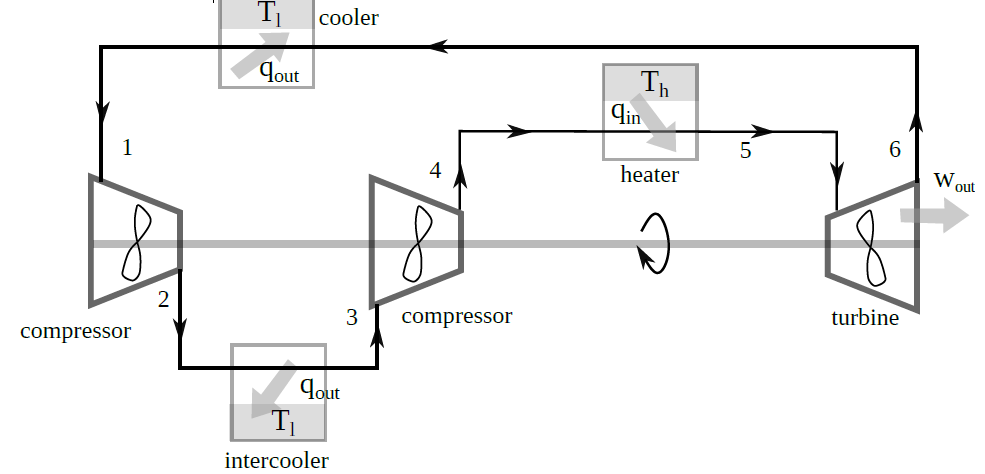
\includegraphics[width=7cm]{figures/cycles/Brayton_Cycle_Intercool.png} }}% 
    \qquad
    \subfloat[\centering]{{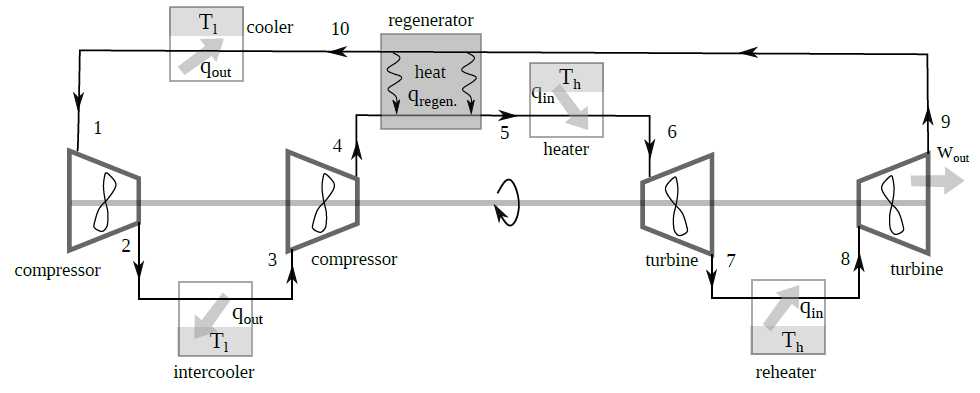
\includegraphics[width=7cm]{figures/cycles/Brayton_Cycle_RIR.png} }}%
    \caption{(a) Simple Brayton Cycle, (b) Brayton Cycle with Regeneration, (c) Brayton Cycle with Intercooling, (d) Brayton Cycle with Regeneration, Intercooling, and Reheating (RIR) \cite{shahbazi_2023}.}%
    \label{fig:cycles}%
\end{figure}

\section{Analysis Methodology and Derivations}
Because the power cycles are evaluated as power plant designs, net work out is first among our evaluation criteria with first law efficiency being the second. These criteria allow for high power production while maintaining a low cost. Second law efficiency and exergy destroyed are used as supporting evidence for our selection of the optimal cycle.   \\

First law efficiencies are plotted versus net work out for each cycle and working gas to find the highest work out with a reasonably high efficiency. To show the effect of inefficiency in the components, turbine and compressor efficiencies are also varied between 80 and 100 percent. Ribbon plots are used to show the effect of this variation on the net work out and first law efficiency with the dashed and solid lines demonstrating the 80 and 100 percent efficiency bounds, respectively. The derivation of the equations for the net work out, first and second law efficiencies, and exergy destroyed for each cycle are detailed below. 

\subsection{Property Relations}

\subsubsection{Ideal Gas Relations and Definitions}

\vspace{-5mm}

\begin{multicols}{3}
  \begin{align*}
    \kappa=\frac{c_p}{c_v}\\
  \end{align*}
  \vspace{1mm}
  \begin{align*}
    \alpha=\frac{\kappa-1}{\kappa} \\
  \end{align*}
  \vspace{1mm}
  \begin{align*}
    \Delta s = c_{v} ln \left( \frac{T_2}{T_1} \right) - R ln\left(  \frac{p_2}{p_1} \right)\\
  \end{align*}
\end{multicols}

\vspace{-15mm}

\subsubsection{Isentropic Relations}

\vspace{-5mm}

\begin{multicols}{2}
    \begin{align*}
      \frac{p_2}{p_1}=r_p \\
    \end{align*}
    \vspace{1mm}
    \begin{align*}
        \frac{T_2}{T_1}=r_p^\alpha
    \end{align*}
\end{multicols}

\subsection{First and Second Law Specializations}
The First Law of Thermodynamics, in its expanded form, is

\begin{align*}
    \sum_{in} \left[ \dot{Q} + \dot{W} + \dot{m}\left(h + \frac{v^{2}}{2} + gz\right) \right] - \sum_{out} \left[\dot{Q} + \dot{W} + \dot{m}\left(h + \frac{v^{2}}{2} + gz\right) \right] = \frac{\partial}{\partial t} \left[m\left(u + \frac{v^{2}}{2} + gz\right)\right]
\end{align*}
\\
\noindent Ignoring the start up period, every process in the Brayton Cycle is steady; therefore, the First Law can be rewritten in terms of specific quantities as follows:
\\
\begin{equation}
    \sum_{in} \left[ {q} + w + \left(h + \frac{v^{2}}{2} + gz\right) \right] - \sum_{out} \left[q + w + \left(h + \frac{v^{2}}{2} + gz\right) \right] = 0
    \label{eq:1st_law} \\
\end{equation}
\\
\noindent The following are specializations of Equation (\ref{eq:1st_law}) for isentropic turbines and compressors.

\vspace{-5mm}

\begin{multicols}{2}
  \begin{align*}
    w_{turb,s} &= h_{in} - h_{out} \\
    w_{turb,s} &= c_{p}\left(T_{in} - T_{out}\right) \\
    w_{turb,s} &= c_{p}T_{in}\left(1 - r_{p}^{-\alpha}\right)
  \end{align*}
  \vspace{1mm}
  \begin{align*}
    w_{comp,s} &= h_{out} - h_{in} \\
    w_{comp,s} &= c_{p}\left(T_{out} - T_{in}\right) \\
    w_{comp,s} &= c_{p}T_{in}\left(r_{p}^{\alpha} - 1\right)
  \end{align*}
\end{multicols}
\noindent Likewise, the specialization of Equation (\ref{eq:1st_law}) for $q_{out}$ and $q_{in}$ is shown below.
\vspace{-5mm}

\begin{multicols}{2}
  \begin{align*}
    q_{out} &= h_{in} - h_{out} \\
    q_{out} &= c_{p}\left(T_{in} - T_{out}\right) \\
  \end{align*}
  \vspace{1mm}
  \begin{align*}
    q_{in} &= h_{out} - h_{in} \\
    q_{in} &= c_{p}(T_{out} - T_{in})  
  \end{align*}
\end{multicols}

\vspace{-5mm}

\noindent The entropy balance equation, in its expanded form, is
\begin{align*}
   \left[\int\sum \frac{Q}{T} + \dot{m}s \right]_{in} - \left[\int\sum \frac{Q}{T} + \dot{m}s \right]_{out} + S_{gen} = \frac{\partial S_{sys}}{\partial t}
\end{align*}
\\
\noindent Due to the steady nature of the Brayton Cycle, the entropy balance equation, written in terms of specific quantities, is as follows:
\begin{equation}
   \left[\int\sum \frac{q}{T} + s \right]_{in} - \left[\int\sum \frac{q}{T} + s \right]_{out} + s_{gen} = 0
       \label{eq:2st_law} \\
\end{equation}
\\
\noindent The following are specializations of Equation (\ref{eq:2st_law}) for $q_{in}$, $q_{out}$, and the whole cycle.


\begin{align*}
    s_{gen} &= \left(s_{out}-s_{in} \right) - \frac{q_{in}}{T_{h}} \,\, \iff  s_{gen} =  c_{p}\left(ln\frac{T_{out}}{T_{in}} - \frac{T_{out}-T_{in}}{T_{h}} \right)\\     
    s_{gen} &= \left(s_{out}-s_{in}\right) + \frac{q_{out}}{T_{L}}      \iff  s_{gen} = c_{p} \left(\frac{T_{in} - T_{out}}{T_{L}} + ln\frac{T_{out}}{T_{in}} \right) \\
    s_{gen} &= \frac{q_{out}}{T_{L}} - \frac{q_{in}}{T_{H}} 
\end{align*}
\subsection{Net Work Out}

Given the isentropic efficiencies of the turbine and compressor, $w_{in,act}$ and $w_{out,act}$ can be found as follows:

\begin{align*}
    \eta_{s,turb} = \frac{w_{out,act}}{w_{out,ideal}} \hspace{1cm} 
    \eta_{s,comp} = \frac{w_{in,ideal}}{w_{in,act}} 
\end{align*}
\vspace{2mm}
\begin{align*}
    w_{out,act} &= \eta_{s,turb}w_{w_{out,ideal}} \iff w_{out,act} = c_{p}\eta_{s,turb}T_{in}\left(1-r_{p}^{-\alpha}\right) \\
    w_{act,in} &= \frac{1}{\eta_{s,comp}}{w_{in,ideal}} \, \iff \hspace{0.145cm} w_{in,act} = \frac{c_{p}T_{in}}{\eta_{s,comp}}\left(r_{p}^{\alpha} - 1\right)
\end{align*}
\vspace{2mm}

\subsubsection{Simple Brayton Cycle} 
\noindent Utilizing isentropic temperature relations and relating the previous to the work in and out of the cycle:

\vspace{-5mm}


\begin{align*}
    w_{out,act} &= c_{p}\eta_{s,turb}T_{3}\left(1-r_{p}^{-\alpha}\right) \\
    w_{in,act} &= \frac{c_{p}T_{1}}{\eta_{s,comp}}\left(r_{p}^{\alpha} - 1\right)
\end{align*}

\vspace{1.5mm}

\begin{equation}
    w_{net} = c_p[\eta_{s,turb}T_3(1-r_p^{-\alpha})-\frac{T_1}{\eta_{s,comp}}(r_p^\alpha-1)] \\
    \label{eq:simple_w_net}
\end{equation}

\subsubsection{Brayton Cycle with Regeneration} 
The outlet and inlet temperatures of the turbine and compressor in the Brayton Cycle with Regeneration are identical to the Simple Brayton Cycle; therefore, the net work of this cycle is the same as the simple cycle (\ref{eq:simple_w_net}). This implies that the purpose of adding regeneration is to modify the efficiency of the cycle, not to increase the net work of the turbine.

\subsubsection{Brayton Cycle with Intercooling} 
The equation for the net work for this cycle can be derived through the following:

\begin{align*}
    r_{p,1} &= \sqrt{r_{p}} \\ 
    w_{comp} &= c_p T_{min}(r_{p,1}^\alpha-1) \\
    w_{turb} &= c_p T_{max}(1-r_{p,1}^{-\alpha}) \\
    w_{net} &= \eta_{turb} w_{turb}-2\frac{w_{comp}}{\eta_{comp}} 
\end{align*}

\begin{equation}
    w_{net} = c_p[\eta_{turb}T_{max}(1-r_{p,1}^{-\alpha})-2\frac{T_{min}}{\eta_{comp}}(r_{p,1}^\alpha-1)] 
    \label{eq:w_net_rir}
\end{equation}

\subsubsection{Brayton Cycle with Regeneration, Intercooling, and Reheating} 

Analyzing the temperature relations we find:

\vspace{-5mm}

\begin{multicols}{2}
  \begin{align*}
    T_{in} &= T_1=T_3=T_{min} \\
    T_{out} &= T_2=T_4 \\
    T_{out} &= T_{in}r_{p,1}^\alpha \\
  \end{align*}
  \vspace{1mm}
  \begin{align*}
    T_{in} &=T_6=T_8=T_{max} \\
    T_{out} &=T_7=T_9 \\
    T_{out} &= T_{in}r_{p,1}^{-\alpha} \\
  \end{align*}
\end{multicols}

\vspace{-10mm}

\noindent Based on the temperatures, we can find the following work and efficiency relations:

\vspace{-2.5mm}

\begin{align*}
    w_{net} &= 2\eta_{turb}w_{turb}-2\frac{w_{comp}}{\eta_{comp}} 
\end{align*}


\begin{equation}
    w_{net} = 2c_p[\eta_{turb}T_{max}(1-r_{p,1}^{-\alpha})-\frac{T_{min}}{\eta_{comp}}(r_{p,1}^\alpha-1)] 
\end{equation}

\subsection{Thermal Efficiency}

\subsubsection{Simple Brayton Cycle} 

\vspace{-5mm}

\begin{multicols}{2}
  \begin{align*}
   \eta_{Th} &= \frac{w_{net}}{q_H}\\
   q_H &= c_p(T_3-T_2)
  \end{align*}
  \vspace{1mm}
  \begin{align*}
    T_2 &= T_1r_p^\alpha\\
    q_H &= c_p(T_3-T_1r_p^\alpha)
  \end{align*}
\end{multicols}

\vspace{-5mm}

\begin{equation}
    \eta_{Th}=\frac{w_{net}}{c_p(T_3-T_1r_p^\alpha)}
\end{equation}

\subsubsection{Brayton Cycle with Regeneration} 

First, we can determine the heat into the system:

\vspace{-5mm}

\begin{multicols}{2}
  \begin{align*}
    T_{2} &= T_{1}r_{p}^\alpha\\
  \end{align*}
  \vspace{-1mm}
  \begin{align*}
    T_4 &= T_3r_p^{-\alpha}\\
  \end{align*}
\end{multicols}
\vspace{-10mm}
\begin{align*}
    \epsilon = \frac{h_5-h_2}{h_4-h_2} = \frac{T_5-T_2}{T_4-T_2} \iff T_5 = \epsilon(T_4-T_2)+ T_2
\end{align*}
\vspace{1mm}
\begin{align*}
    q_H &= T_3-T_5 \iff q_H = T_3-\epsilon(T_4-T_2) - T_2
\end{align*}
\vspace{2mm}

\noindent Since $\eta_{Th} = \frac{w_{net}}{q_H}$, we know the First Law Efficiency if we know the equation for net work. For this cycle, it is Equation (\ref{eq:simple_w_net}).

\begin{equation}
    \eta_{Th}=\frac{w_{net}}{c_p[T_3-\epsilon(T_3r_p^{-\alpha}-T_1r_p^\alpha)-T_1r_p^\alpha]}
\end{equation}

\subsubsection{Brayton Cycle with Intercooling} 

\vspace{-5mm}

\begin{multicols}{2}
  \begin{align*}
   \eta_{Th} &= \frac{w_{net}}{q_H}\\
    T_4 &= T_2\\
    q_H &= c_p(T_{6}-T_2)\\
  \end{align*}
  \vspace{1mm}
  \begin{align*}
    T_2 &= \frac{T_1r_p^\alpha}{\eta_{comp}}\\
    q_H &= c_p(T_{6}-\frac{T_1r_p^\alpha}{\eta_{comp}})
  \end{align*}
\end{multicols}

\vspace{-10mm}

\begin{equation}
    \eta_{Th}=c_p(T_{6}-\frac{T_1r_p^\alpha}{\eta_{comp}})
\end{equation}

\subsubsection{Brayton Cycle with Regeneration, Intercooling, and Reheating} 

Analyzing the temperature relations we find:

\vspace{-5mm}

\begin{multicols}{2}
  \begin{align*}
    T_{min} &= T_1 = T_3 \\
    T_2 &= T_4 = \frac{T_{min}r_{p,1}^\alpha}{\eta_{comp}} \\
  \end{align*}
  \begin{align*}
    T_{max} &= T_6 = T_8 \\
     T_7 &= T_9= T_{max}r_{p,1}^{-\alpha}\eta_{turb} \\
  \end{align*}
\end{multicols}
\vspace{-7.5mm}
\begin{align*}
    \epsilon &= \frac{h_5-h_4}{h_9-h_4}=\frac{T_5-T_4}{T_9-T_4} \iff T_5 = \epsilon(T_9-T_4)+T_4\\ 
\end{align*}
\noindent Determine the heat transfered:

\vspace{5mm}


\begin{align*}
    q_{H,1} & =c_p(T_{6}-T_5) \iff q_{H,1} =c_p(T_{6}-\epsilon(T_9-T_4)+T_4)\\
    q_{H,2} &=c_p(T_{6}-T_7) \iff q_{H,2} = c_pT_{6}(1-r_{p,1}^{-\alpha})\\
    q_H &= q_{H,1}+q_{H,2} \,\, \iff  q_H = c_p(T_{max}-T_5)+c_pT_{max}(1-r_{p,1}^{-\alpha})\\
\end{align*}



\noindent From this and Equation (\ref{eq:w_net_rir}) can determine that:

\begin{equation}
    \eta_{th}=\frac{w_{net}}{c_p(T_{max}-T_5)+c_pT_{max}(1-r_{p,1}^{-\alpha})}
\end{equation}

\subsection{Second Law Efficiency}

If the First Law Efficiency is known for a cycle, it is trivial to determine the Second Law Efficiency. This can be done through the following:

\begin{multicols}{2}
  \begin{align*}
    T_{avg} &=\frac{T_a-T_b}{\ln{\frac{T_a}{T_b}}} \\
  \end{align*}
  \begin{align*}
    \eta_{Th,rev} &= 1 - \frac{T_L}{T_{max,avg}}\\
    \eta_{II} &= \frac{\eta_{Th}}{\eta_{Th, rev}} \\
  \end{align*}
\end{multicols}
\vspace{-15mm}
\begin{equation}
    \eta_{II}=\frac{T_{max}\eta_{Th}}{T_{max}-T_{min}}
\end{equation}


\section{Analysis of Cycles}

\subsection{Simple Brayton Cycle}

The Simple Brayton Cycle provides a baseline for us to compare our modified Brayton Cycles against and to observe the performance of the working gasses. Given the graph shown in Figure (\ref{fig:simple_brayton_cycle}), the gas that produces the highest net work out is Hydrogen. Its net work out is  7040 $\frac{kJ}{kg}$ with a first law efficiency of 55.7\%. This occurs at a $r_{p}$ value of $16.6$. The next highest net work out is produced with Helium as the working gas and is far less at $2555$ $\frac{kJ}{kg}$ with a similar first law efficiency of $55.6\%$. It is important to note that for this study we considered compression ratios in the following range: $1 \leq r_p \leq 60$.


\begin{figure}[]%
    \centering
    \subfloat[\centering]{{\includesvg[width=6.5cm]{figures/simple/simple_work_rp.svg}}}%
    \qquad
    \subfloat[\centering]{{\includesvg[width=6.5cm]{figures/simple/simple_nth_rp.svg} }}%
    \qquad
    \subfloat[\centering]{{\includesvg[width=6.5cm]{figures/simple/simple_work_nth.svg} }}%
    \qquad
    \subfloat[\centering]{{\includesvg[width=6.5cm]{figures/simple/simple_nii_rp.svg} }}%
    \caption{Simple Brayton Cycle: (a) Net Work Out vs. Compression Ratio, (b) Thermal Efficiency vs. Compression Ratio, (c) Net Work Out vs. Thermal Efficiency, (d) Second Law Efficiency vs. Compression Ratio. In Plot (b) Argon and Helium are overlaid and Hydrogen and air are overlaid. This is a result of their similar $\kappa$ values. In Plot (d) all four gases are overlaid because the simple cycle is fully reversible. } %
    \label{fig:simple_brayton_cycle}%
\end{figure}

\subsection{Brayton Cycle with Regeneration}

The graphs shown in Figure (\ref{fig:Brayton_Cycle_Regeneration}) show the Brayton Cycle with regeneration to have the same work produced as the Simple Brayton cycle but with an efficiency inversely proportional to the regenerative effectiveness. Ultimately, the cycle was most efficient with no regenerative effectiveness and least efficient with ideal regenerative effectiveness. This shows that regeneration has no benefit by itself and is inferior to the simple cycle. 

\begin{figure}%
    \centering
    \subfloat[\centering]{{\includesvg[width=6.5cm]{figures/regen/regen_work_rp.svg}}}%
    \qquad
    \subfloat[\centering]{{\includesvg[width=6.5cm]{figures/regen/regen_nth_rp.svg} }}%
    \qquad
    \subfloat[\centering]{{\includesvg[width=6.5cm]{figures/regen/regen_work_nth.svg} }}%
    \qquad
    \subfloat[\centering]{{\includesvg[width=6.5cm]{figures/regen/regen_nii_rp.svg} }}%
    \caption{Brayton Cycle with Regeneration: (a) Net Work Out vs. Compression Ratio, (b) Thermal Efficiency vs. Compression Ratio, (c) Net Work Out vs. Thermal Efficiency, (d) Second Law Efficiency vs. Compression Ratio. In Plots (b) and (d) Argon and Helium are overlaid and Hydrogen and air are overlaid. This is a result of their similar $\kappa$ values.}%
    \label{fig:Brayton_Cycle_Regeneration}%
\end{figure}


\subsection{Brayton Cycle with Intercooling} 

The Brayton Cycle with intercooling performs better than the simple cycle. Figure (\ref{fig:Brayton_Cycle_Intercooling}) shows that, for the intercooling cycle, Hydrogen produces a net work out of 8610 $\frac{kJ}{kg}$ with a thermal efficiency of 57.2\%. This occurs at a $r_{p}$ value of 42.9. This work is higher than that of the simple cycle with a comparable thermal efficiency level. 

\begin{figure}%
    \centering
    \subfloat[\centering]{{\includesvg[width=6.5cm]{figures/intercool/intercool_work_rp.svg}}}%
    \qquad
    \subfloat[\centering]{{\includesvg[width=6.5cm]{figures/intercool/intercool_nth_rp.svg} }}%
    \qquad
    \subfloat[\centering]{{\includesvg[width=6.5cm]{figures/intercool/intercool_work_nth.svg} }}%
    \qquad
    \subfloat[\centering]{{\includesvg[width=6.6cm]{figures/intercool/intercool_nii_rp.svg} }}%
    \caption{Brayton Cycle with Intercooling: (a) Net Work Out vs. Compression Ratio, (b) Thermal Efficiency vs. Compression Ratio, (c) Net Work Out vs. Thermal Efficiency, (d) Second Law Efficiency vs. Compression Ratio. In Plots (b) and (d) Argon and Helium are overlaid and Hydrogen and air are overlaid. This is a result of their similar $\kappa$ values.}%
    \label{fig:Brayton_Cycle_Intercooling}%
\end{figure}


\begin{figure}%
    \centering
    \subfloat[\centering]{{\includesvg[width=6.5cm]{figures/rir/rir_work_rp.svg}}}%
    \qquad
    \subfloat[\centering]{{\includesvg[width=6.5cm]{figures/rir/rir_nth_rp.svg} }}%
    \qquad
    \subfloat[\centering]{{\includesvg[width=6.5cm]{figures/rir/rir_work_nth.svg} }}%
    \qquad
    \subfloat[\centering]{{\includesvg[width=6.5cm]{figures/rir/rir_nii_rp.svg} }}%
    \caption{Brayton Cycle with Regeneration, Intercooling, and Reheating: (a) Net Work Out vs. Compression Ratio, (b) Thermal Efficiency vs. Compression Ratio, (c) Net Work Out vs. Thermal Efficiency, (d) Second Law Efficiency vs. Compression Ratio. In Plots (b) and (d) Argon and Helium are overlaid and Hydrogen and air are overlaid. This is a result of their similar $\kappa$ values.}%
    \label{fig:Brayton_Cycle_RIR}%
\end{figure}

\subsection{Brayton Cycle with Regeneration, Intercooling, and Reheating}

The RIR Brayton Cycle performs far better than any other cycle. Hydrogen produces the greatest max net work out at 13080 $\frac{kJ}{kg}$ as evident in Figure (\ref{fig:Brayton_Cycle_RIR}). The max net work out is 4467 $\frac{kJ}{kg}$ greater than the max net work out of the Brayton Cycle with intercooling. The thermal efficiency of 52.7\% is the lowest out of the four cycle designs analyzed; however, the difference in thermal efficiency is relatively small compared to the gain in the $W_{out,net,max}$.

\section{Exergy Analysis}

\subsection{Exergy Derivation}

Using the definition that $\Phi_{dest} = T_{0} S_{gen}$, we can determine the exergy destroyed for the RIR Brayton Cycle:

\begin{align*}
    \Phi_{dest,q_{in}} &= T_{0}\left[ c_pln \left( \frac{T_{out}}{T_{in}} \right) + \frac{c_p}{T_0}\left(T_{in} - T_{out}\right) \right] \\
    \Phi_{dest,q_{out}} &= T_{0} \left[ c_pln \left( \frac{T_{out}}{T_{in}} \right) - c_p\left(T_{out} - T_{in}\right) \right] \\
    \Phi_{dest,turb} &= (1 - \eta_t)c_p(T_{in} - T_{out})\\
    \Phi_{dest,comp} &= \left(\frac{1}{\eta_c} - 1\right)c_p(T_{out}-T_{in})\\
    \Phi_{dest,regen} &= T_0 c_p \left[ln\left(\frac{T_{cold,out}}{T_{hot,in}}\right) + ln\left( \frac{\epsilon(T_{hot,in} - T_{cold,in}) + T_{cold,in}}{T_{cold,in}}\right) \right]\\
\end{align*} 
Invoking the additive property of exergy yields the following equation: \\

\begin{equation}
    \Phi_{dest,tot} = \Phi_{dest,q_{in}} + \Phi_{dest,q_{out}} + \Phi_{dest,turb} + \Phi_{dest, comp} + \Phi_{dest, regen} \\
    \label{Exergy_Dest}
\end{equation}

\subsection{Exergy Destroyed}

To see which components are most critical to the Second Law Efficiency, $\Phi_{dest}$ was derived and can be seen in Equation (\ref{Exergy_Dest}). Then individual plots of $\eta_{s,t}$ vs $r_p$, $\eta_{s,c}$ vs $r_p$, and $\epsilon$ vs $r_p$ were made, for the RIR cycle, to see which components affect Second Law Efficiency the most. As shown in Figure (\ref{fig:Exergy_Plots}), increasing the isentropic turbine efficiency is imperative to developing an ideal cycle. The second most important parameter contributing to the Second Law Efficiency is the isentropic efficiency of the compressor. Lastly, regenerative effectiveness can be varied to increase $\eta_{II}$. As shown in Figure (\ref{fig:Exergy_Plots}) Plot (c), the regenerative effectiveness is an order of magnitude less impactful on the total $\Phi_{dest}$ than the other parameters; therefore, it is critical to decrease efficiencies losses in the turbine and compressor.



\begin{figure}%
    \centering
    \subfloat[\centering]{{\includesvg[width=6.5cm]{figures/rir_exergy/rir_exergy_qin_turb.svg}}}%
    \qquad
    \subfloat[\centering]{{\includesvg[width=6.5cm]{figures/rir_exergy/rir_exergy_qin_comp.svg}}}%
    \qquad
    \subfloat[\centering]{{\includesvg[width=6.5cm]{figures/rir_exergy/rir_exergy_qin_regen.svg}}}%
    \qquad
    \caption{Exergy Analysis of Brayton Cycle with Regeneration, Intercooling, and Reheating with : (a) Pressure Ratio vs. Exergy Destroyed, Turbine with varying efficiency (dashed line: $\eta_t$ = 0.8, solid line: $\eta_t$ = 1.0), (b) Pressure Ratio vs. Exergy Destroyed, Compressor with varying efficiency (dashed line: $\eta_c$ = 0.8, solid line: $\eta_c$ = 1.0), (c) Pressure Ratio vs. Exergy Destroyed, Regeneration with varying effectiveness (dashed line: $\epsilon$ = 0.8, solid line: $\epsilon$ = 1.0)}%
    \label{fig:Exergy_Plots}%
\end{figure}




\section{Proposed Optimal Design}

Given the analysis above, we propose a Brayton Cycle with Regeneration, Intercooling, and Reheating with Hydrogen as the working fluid. For an optimal design the power cycle should operate under the following conditions: the low temperature reservoir is $283K$, the high temperature reservoir is $1620K$, the $T_{min}$ of the working gas is $313K$, and the $T_max$ of the working fluid is $1590K$. Under these conditions, the RIR Brayton Cycle produced far more work than any other cycle while maintaining both a first and second law efficiencies that was comparable to that of the other cycles.
\\

A compression ratio of 60 was selected and represents an upper bound on reasonable compression ratios for this type of cycle. While the maximum work out for this design occurs at a pressure ratio of approximately 280, having a large compression ratio comes with the problems of material strength and the turbulency of the fluid, which are not modeled nor considered in this analysis.  We propose that further work be done on investigating the effects of high pressure ratios on the work generated. Ultimately, this design generates the optimal work out for the Brayton Cycle designs evaluated. 

\newpage
\phantomsection   % 
\printbibliography[heading=bibintoc, title={References}]

\begin{comment}
\newpage
\section{Appendix}
\indent
\lipsum[1]
\end{comment}

\end{document}

\begin{comment}
Simple
+=================+
$Ar$
work out net max: 255.88400884125068
r_p at max: 7.6
η_th: 0.5567796457607569
η_II: 0.46520212126095817
+=================+
$Air$
work out net max: 494.5458049131115
r_p at max: 17.2
η_th: 0.5563996579904366
η_II: 0.46488463279285025
+=================+
$He$
work out net max: 2555.3947332784533
r_p at max: 7.6
η_th: 0.5558098880124631
η_II: 0.4643918664949114
+=================+
$H_2$
work out net max: 7040.261765668311
r_p at max: 16.8
η_th: 0.5565986933304125
η_II: 0.46505093136907816


Intercool
+=================+
$Ar$
work out net max: 312.9504594913933
r_p at max: 14.9
η_th: 0.5721482737433697
η_II: 0.4780429612464308
+=================+
$Air$
work out net max: 604.8369451102567
r_p at max: 44.4
η_th: 0.5721487205751321
η_II: 0.47804333458458226
+=================+
$He$
work out net max: 3125.291936230032
r_p at max: 15.0
η_th: 0.5721139587198397
η_II: 0.4780142902598766
+=================+
$H_2$
work out net max: 8610.350807572822
r_p at max: 42.9
η_th: 0.5721100422572725
η_II: 0.4780110179658766


Regen
+=================+
$Ar$
work out net max: 255.88400884125068
r_p at max: 7.6
η_th: 0.5558521985078093
η_II: 0.46442721788093366
+=================+
$Air$
work out net max: 494.5458049131115
r_p at max: 17.2
η_th: 0.5562326552315737
η_II: 0.46474509817036375
+=================+
$He$
work out net max: 2555.3947332784533
r_p at max: 7.6
η_th: 0.5568218638836493
η_II: 0.46523739546768383
+=================+
$H_2$
work out net max: 7040.261765668311
r_p at max: 16.8
η_th: 0.5560334555832919
η_II: 0.46457866231079037


RIR
+=================+
$Ar$
work out net max: 511.7688047181428
r_p at max: 57.5
η_th: 0.5563161531597088
η_II: 0.46481486259797006
+=================+
$Air$
work out net max: 915.2317128702206
r_p at max: 60.0
η_th: 0.5256928562024132
η_II: 0.4392283979830988
+=================+
$He$
work out net max: 5110.798987308319
r_p at max: 58.1
η_th: 0.5563161638122852
η_II: 0.46481487149844114
+=================+
$H_2$
work out net max: 13076.773273991232
r_p at max: 60.0
η_th: 0.5271101627057893
η_II: 0.4404125899643746

\begin{table}[ht!]
    \centering
    \caption{lorem ipsum}
    \begin{tabular}{c|c|c|c}
        Gas & $Work_{out net max} \, \frac{kJ}{kg}$ & $r_{p} \, $η_{th} \, \% $ $η_{II} \, \% $ \\
        \hline
        Air &  \\
        Argon (Ar) & 511.8 & 57.5 & 55.6 & 46.5\\
        Hydrogen (H2) &  \\
        Helium (He) & 
        \label{tab:gasses}
    \end{tabular}
    \label{tab:my_label2}
\end{table}

\end{comment}